\documentclass[12pt]{article}
\usepackage[utf8]{inputenc}
\usepackage[italian]{babel}
\usepackage{graphicx}
\usepackage{geometry}
\usepackage{url}
\usepackage[hang,flushmargin]{footmisc}
\usepackage{fancyhdr}
\usepackage{lastpage}
\usepackage{footnote}
\usepackage{float}
\usepackage{textcomp}
\usepackage[colorinlistoftodos]{todonotes}
%\usepackage[hidelinks]{hyperref}
\PassOptionsToPackage{hyphens}{url}\usepackage{hyperref}
\hypersetup{colorlinks, linkcolor=black, urlcolor=blue}

%Layout di pagina
\geometry{
	a4paper,
	total={160mm,225mm},
	left=25mm,
	top=25mm
}

%intestazione e piè di pagina
\pagestyle{fancy}
\fancyhf{}
\renewcommand{\headrulewidth}{0.4pt}
\renewcommand{\footrulewidth}{0.4pt}
\setlength\headheight{57pt}
\lhead{Relazione del progetto \textbf{DevSpace}}
\rhead{\nouppercase{\leftmark}}
\lfoot{DevSpace}
\rfoot{Pagina \thepage\ di \pageref{LastPage}}


%\newcommand{\code}[1]{\texttt{#1}}
\interfootnotelinepenalty=10000
\DeclareTextFontCommand{\code}{\ttfamily\hyphenchar\font=45\relax}

\begin{document}

	\begin{titlepage} % Suppresses displaying the page number on the title page
	\begin{center} % Centre everything on the page

		%------------------------------------------------
		%	Headings
		%------------------------------------------------
		
		\textsc{\LARGE Università degli studi di Padova}\\[1.5cm]
		
		\textsc{\Large Corso di Laurea in Informatica}\\[0.5cm]
		
		\textsc{\Large Progetto di Tecnologie Web}\\[0.5cm]
		
		
\includegraphics[scale=1.5]{img/logoFinal.eps}
		
		\textsc{\large a.a. 2018/2019}\\[0.5cm] % Minor heading such as course title
		
		%------------------------------------------------
		%	Title
		%------------------------------------------------
		
		{\huge\ Relazione}\\[0.4cm] % Title of your document
		
		%------------------------------------------------
		%	Author(s)
		%------------------------------------------------
		
	 	\large
			\begin{tabular}{l r}
				\emph{Team:} & \emph{Matricola:} \\
				Giacomo \textsc{Barzon} & 1143164 \\
				Francesco \textsc{De Filippis} & 1143408 \\
				Giacomo \textsc{Greggio} & 1142951 \\
				Michele \textsc{Roverato} & 1143030 \\
			\end{tabular}
	\end{center}
\end{titlepage}
	%----------------------------------------------------------------------------------------
	
	\section*{Informazioni logistiche}
	
	Il sito è accessibile al seguente link:
	\begin{center}
		\url{http://tecweb1819.studenti.math.unipd.it/mroverat/}
	\end{center}
	
	Account non amministratore utilizzabile:
	\begin{itemize}
		\item \textbf{Username}: linus@torvalds.com
		\item \textbf{Password}: git
	\end{itemize}
	
	Account amministratore utilizzabile:
	\begin{itemize}
		\item \textbf{Username}: admin@admin.it
		\item \textbf{Password}: admin
	\end{itemize}

	\newpage
	
	\tableofcontents
	
	\newpage

	\section{Analisi dei requisiti}
		\subsection{Requisiti}
		Lo scopo di questo progetto consiste nel dare vita ad una piattaforma web che offre la possibilità di consultare un archivio di informazioni sugli argomenti del mondo informatico. Gli utenti troveranno le informazioni suddivise nel seguente modo:
		\begin{itemize}
			\item Nella home page sono disponibili delle card che identificano il macroargomento, mostrano una immagine ad esso relativa e vengono elencati i principali sottoargomenti tramite dei link;
			\item Ad ogni argomento è dedicata una pagina che contiene tutti i suoi sottoargomenti e per ciascuno di essi gli articoli associati.
		\end{itemize}
		 L'utente ha inoltre la possibilità di commentare i singoli articoli, interagendo così con gli altri utenti registrati al blog. L'utente ha la possibilità di lasciare un giudizio (pollice in sù/pollice verso) ai commenti degli altri utenti. Gli amministratori dispongono di un pannello amministratore in cui vengono elencate le operazioni che possono compiere, tra cui aggiornare la piattaforma con nuovi contenuti (eventualmente migliorando contenuti già esistenti), sospendere un account utente e nominare nuovi amministratori.
		Devono inoltre occuparsi di moderare l'ambiente sfruttando la possibilità di eliminare eventuali commenti inopportuni.
	\subsection{Target di utenza}
		Il sito è rivolto ad un pubblico che ha dimestichezza con la tecnologia e certamente con l'utilizzo di Internet per cercare informazioni. Inoltre può essere consultato da persone che desiderano acquisire delle nozioni sui principali argomenti riguardanti l'informatica, perciò si prevede che la piattaforma verrà raggiunta da utenti con età superiore ai 14 anni (e.g. dagli studi superiori in poi).
		
	\section{Architettura delle informazioni}
	\subsection{Descrizione}
		In questa sezione verrà descritto il modo in cui è stato scelto di gestire le informazioni presentate nel sito. Poiché si tratta di un blog in cui la quantità di contenuti è destinata a crescere nel tempo, è stata adottata un'interfaccia a tre pannelli, navbar, sidebar e contenuto. La spiegazione dettagliata verrà fornita nella sezione \textbf{Usabilità}.
	\subsection{Struttura pagine pubbliche}
		La parte pubblica del sito è accessibile a tutti gli utenti e di seguito verranno descritte le pagine visitabili con le relative funzionalità offerte.
		\begin{itemize}
				\item \textbf{Homepage (index.php)}: si tratta della pagina principale del sito in cui l'utente trova le seguenti informazioni:
				\begin{itemize}
						\item \textbf{Navbar}: parte superiore della pagina in cui viene mostrato il logo del sito e una lista orizzontale di link utili alla navigazione;
						\item \textbf{Header}: sezione sottostante alla navbar composta da immagine di sfondo e nome del sito;
						\item \textbf{Descrizione e Contenuto}: nella parte inferiore dell'header è presente una descrizione del sito, seguita dalla lista dei macroargomenti visualizzati sotto forma di card;
						\item \textbf{Casella di ricerca}: situata prima delle card, permette la ricerca di contenuti specifici che riguardano macroargomenti, sottoargomenti e articoli;
						\item \textbf{Footer}: parte inferiore del sito contenente ulteriori informazioni sulla piattaforma.
				\end{itemize}
			\item \textbf{About (about.php)}: è una pagina che fornisce tutte le informazioni sul sito, ovvero lo scopo dello stesso e gli sviluppatori che lo hanno realizzato. Anche in questa pagina è presente la navbar per la navigabilità, l'header e il footer;
			\item \textbf{Ricerca (search.php)}: in questa pagina vengono visualizzati i risultati di una ricerca avvenuta tramite la casella di ricerca, utile per trovare in modo veloce specifici argomenti e/o articoli;
			\item \textbf{Registrazione (registrazione.php)}: pagina che offre la possibilità di creare un account agli utenti non registrati al blog;
			\item \textbf{Login (login.php)}: pagina che offre la possibilità di effettuare il login agli utenti che sono registrati alla piattaforma;
			\item \textbf{Link Articoli (ArticleLinks.php)}: questa pagina contiene tutti i sottoargomenti, con i relativi link agli articoli, appartenenti ognuno al proprio macroargomento. La pagina è strutturata nel seguente modo:
				\begin{itemize}
					\item Sulla sinistra è presente una sidebar che elenca tutti i macroargomenti e, nella parte superiore, mette a disposizione la casella di ricerca già descritta;
					\item Nel contenuto, a inizio pagina, a seguito della descrizione del macroargomento che è stato selezionato, vengono elencate tramite link le ancore ai sottoargomenti presenti;
					\item Per ciascun sottoargomento, vengono elencati i link degli articoli relativi;
					\item Nella parte superiore è presente la navbar già descritta precedentemente, e nella parte inferiore è situato il footer, anch'esso già descritto.
				\end{itemize}
			\item \textbf{Articolo (ReadArticle.php)}: questa pagina è strutturata nello stesso modo di quella descritta al punto precedente, ma nel contenuto vi è il corpo di un articolo che l'utente ha raggiunto utilizzando uno dei link elencati sotto ciascun sottoargomento della precedente pagina. Inoltre un utente che si è autenticato alla piattaforma può lasciare dei commenti e votare quelli esistenti;
			\item \textbf{Account (profile.php)}: in questa pagina l'utente può visualizzare le sue informazioni personali, ed eventualmente le può modificare;
		\end{itemize}
	
	\subsection{Struttura pagine privata}
	La parte privata del sito è accessibile ai soli account amministratori della piattaforma. Di seguito verranno descritte le pagine di interesse con le relative funzionalità offerte.
	\begin{itemize}
		\item \textbf{Link Articoli (ArticleLinks.php)}: questa pagina, già descritta, presenta un aspetto diverso per l'utente amministratore, il quale può:
		\begin{itemize}
			\item Aggiungere un nuovo sottoargomento;
			\item Eliminare un sottoargomento esistente;
			\item Scrivere un nuovo articolo;
			\item Modificare un articolo esistente;
			\item Eliminare un articolo esistente.
		\end{itemize}
		\item \textbf{Articolo (ReadArticle.php)}: la pagina, già descritta nella sezione precedente, permette ad un amministratore di eliminare i commenti degli utenti, nel caso in cui non siano pertinenti;
		\item \textbf{Scrivi Articolo (writeArticle.php)}: questa pagina è dedicata alla gestione di un singolo articolo, in particolare l'amministrare può modificare il contenuto di un articolo già esistente, oppure scriverne uno nuovo;
		\item \textbf{Strumenti (adminTools.php)}: in questa pagina l'utente amministratore visualizza una lista delle operazioni che può compiere, ovvero:
			\begin{itemize}
				\item Creare un nuovo macroargomento;
				\item Aggiungere un nuovo amministratore;
				\item Gestire utenti sospesi ovvero sospenderli oppure revocare la sospensione.
			\end{itemize}
		\item \textbf{Gestione argomenti (manageArguments.php)}: questa pagina permette all'amministratore di creare un nuovo macroargomento e di eliminare quelli esistenti;
		\item \textbf{Aggiunta amministratore (addAdmin.php)}: in questa pagina un utente amministratore può aggiungere un nuovo utente al gruppo dei moderatori del sito fornendo il suo indirizzo email. Inoltre può visualizzare la lista degli attuali amministratori del sito. Nella sezione \textbf{Sviluppo} verrà approfondita questa funzionalità.
		\item \textbf{Sospensione account (manageUsers.php)}: in questa pagina un utente amministratore può sospendere un utente, inserendo il suo nickname, restringendo così le sue attività sulla piattaforma, oppure revocare la sospensione ad utenti attualmente sospesi.
	\end{itemize}

	\section{Usabilità}
	\subsection{Introduzione}
	Essendo il sito rivolto ad un pubblico potenzialmente vario, è stato adottato lo schema a tre pannelli il quale, a nostro parere, permette una buona navigabilità data la natura della piattaforma. Inoltre data la struttura gerarchica dei contenuti, abbiamo scelto la suddivisione in macroargomenti, sottoargomenti e articoli per garantire un buon equilibrio tra ampiezza e profondità al fine da non creare sovraccarico cognitivo all'utente; infatti una struttura con solo tre livelli (compresi gli articoli) è, a nostro parere, facile da usare e soprattutto da ricordare.
	\subsection{Layout e design}
	Tutte la pagine che presentano i contenuti, quindi presumibilmente le più visitate, sono dotate di una sidebar che offre un modo intuitivo e veloce per navigare attraverso macroargomenti, sottoargomenti (con searchbar annessa per cercare velocemente contenuti), una navbar che permette di spostarsi in altre aree della piattaforma con un solo click e un footer che fornisce informazioni aggiuntive sul sito.
	\subsection{Scroll verticale}
	Poiché il sito è destinato alla raccolta di contenuti, è possibile che nel tempo questi crescano, generando così delle pagine o sezioni potenzialmente lunghe (soprattutto la sidebar e la pagina con i link agli articoli). Su mobile inoltre, questo tipo di situazione è sentita maggiormente date le dimensioni degli schermi dei dispositivi mobili. L'unico accorgimento per ovviare a questo problema, non tanto per lo scroll necessario alla discesa della pagina quanto alla risalita, è stato l'introduzione di un pulsante che permetta di tornare all'inizio della pagina. Tuttavia esistono oggigiorno moltissimi siti e piattaforme che fanno uso di strutture simili per la presentazione di una grande mole di contenuti, perciò riteniamo che l'utente medio giunto sul nostro sito trovi familiare e semplice questo tipo di layout e modalità di navigazione.
	
	\subsection{Favicon}
	Tutte le pagine sono dotate di favicon che permettono la facile individuazione del sito tra le schede del browser o nei preferiti. Per generare le favicon in diversi formati è stato utilizzato il tool offerto al seguente link:
	\begin{center} 
		\url{https://www.favicon-generator.org/} 
	\end{center}
	
	\subsection{Gestione dell'errore 404}
	E' stato previsto un apposito reindirizzamento a una pagina di errore nel caso in cui venga richiesto il reperimento, da parte dell'utente, di una pagina non esistente, non raggiungibile senza permessi di amministratore oppure senza aver effettuato il login.
	All'interno di questa pagina è stato inserito un apposito messaggio di errore con link annesso per poter tornare alla home page. Tuttavia non è stato possibile configurare il file \emph{.htaccess} presente nel server di deploy in modo adeguato, pertanto il redirect a questa pagina non funzionerà. Per poter visualizzare come è stata realizzata tale pagina, è possibile accedervi al seguente indirizzo: \url{http://tecweb1819.studenti.math.unipd.it/mroverat/errore.php?errore=404}.

	\subsection{Sidebar}
	La sidebar come già accennato è pensata per offrire un modo semplice ed intuitivo per navigare tra i contenuti del sito, pertanto costituisce un elemento cruciale all'interno della nostra piattaforma. Nella sidebar è presente per prima cosa una casella di ricerca, la quale permette di cercare immediatamente dei contenuti specifici invece di navigare per le varie voci presenti più in basso. Sotto la casella di ricerca vi è una lista di voci che rappresentano i macroargomenti, e ciascuna di queste voci si può espandere per visualizzare i rispettivi sottoargomenti, i quali sono link àncora verso la parte centrale della pagina che mostra i sottoargomenti con relativi articoli.

	\subsection{Visualizzazione sotto-argomenti e relativi articoli}
	Per minimizzare il numero di click che l'utente deve effettuare per raggiungere un articolo, il quale non dovrebbe essere superiore a 3 o 4, si è deciso di visualizzare all'interno di un unica pagina tutti i sotto-argomenti ed i relativi articoli ad essi associati. Infatti sia nella sidebar che nelle card presenti all'interno della home sono elencati, per ogni argomento, le àncore che puntano al sotto-argomento specifico nella pagina \textbf{ArticleLinks}. L'alternativa sarebbe stata quella di creare due pagine separate per argomenti e sotto-argomenti, tuttavia abbiamo ritenuto che questa scelta avrebbe rallentato notevolmente la navigazione aumentando considerevolmente il numero di click necessari per spostarsi da articolo ad articolo. Inoltre riteniamo che l'implementazione da noi effettuata non generi problemi di usabilità o accessibilità.

	\subsection{Minificazioni}
	I file .css e .js generalmente vengono minificati al fine di ridurre il loro peso complessivo e quindi velocizzare la richiesta della risorsa al server. Per questioni di leggibilità non è stato fatto, eccetto per le librerie JavaScript, poiché non sviluppate da noi, che abbiamo utilizzato per gestire lo stile della scrollbar situata nella sidebar.
	
	\subsection{Media queries}
	Per garantire la stessa esperienza su tutti i dispositivi si è fatto uso di media queries, in particolare abbiamo individuato due \emph{breakpoint} che ci hanno permesso di adottare una sufficiente suddivisione delle regole css relative ad ampie categorie di dispositivi differenti; 1276px e 768px.
	Per quanto riguarda la possibilità di stampare le pagine del sito, abbiamo scritto un foglio di stile \emph{print.css} che, in fase di stampa, riadatta i contenuti laddove possibile e si occupa di rimuovere gli elementi di non utilità per un documento su carta, per esempio navbar e sidebar in quanto elementi prettamente di navigabilità più che di informazione.

	\section{Accessibilità}
	\subsection{Introduzione}
	Affinché il sito raggiunga la vasta gamma di utenti per cui è stato progettato, particolare attenzione è stata posta sul fattore accessibilità seguendo i principi fondamentali descritti dal WCAG 2.0. In particolare, nel nostro caso specifico, sono stati adottati gli accorgimenti di seguito descritti.
	\subsection{Scelte adottate}
	In questa sezione verranno illustrate le scelte intraprese al fine di rendere il sito accessibile.
	
	\subsubsection{Lingua}
	Poiché gli argomenti trattati nel sito sono di carattere internazionale e in generale gli argomenti di tipo scientifico vengono proposti in lingua inglese, abbiamo deciso di presentare i nostri contenuti in inglese. \\
	Di conseguenza non è stato necessario adottare particolari precauzioni di localizzazione se non utilizzare il tag \code{<html>} con l'attributo \code{lang = "en"};
	\subsubsection{Colori}
	Per quanto riguarda l'utilizzo dei colori per i testi e gli elementi di tutte le pagine, abbiamo assicurato di ottenere un rapporto di contrasto pari 7:1 tra un elemento in foreground e uno in background, rendendo così il sito conforme ai livelli di accessibilità AAA del WCAG 2.0. 
	\subsubsection{Link}
	Sono stati uniformati i link presenti all'interno del sito web, in modo da renderli facilmente riconoscibili da qualsiasi tipologia di utente. La maggior parte dei link è facilmente riconoscibile da una particolare tonalità di blu, e dalla caratteristica sottolineatura diventata ormai uno standard all'interno del web. Gli unici link che fanno eccezione a queste regole sono quelli presenti all'interno della sidebar per questioni estetiche e di contrasto. Il team ritiene tuttavia che siano ugualmente riconoscibili grazie alla notevole diffusione all'interno del web di sidebar dalla struttura simile.
	Come si può notare navigando tra le pagine del sito, non è stata prevista la gestione dei link visited perché secondo il team era sufficiente l'utilizzo dei breadcrumb sia nel menù situato sulla navbar (che ha poche voci e molto basilari) sia nella sidebar (anch'essa dotata di breadcrumb). Essendo quest'ultima utilizzata per navigare i contenuti del sito l'utente potrebbe, dopo poco tempo di navigazione, aver visitato molte delle voci (o quasi tutte) rendendo poco utile il vantaggio offerto dai link visited.
	\newpage
	\subsubsection{JavaScript}
	Il sito risponde bene in caso di assenza di JavaScript in quanto non è stato utilizzato per alterare la struttura della pagina, ma solo per offrire una migliore esperienza d'uso tramite alcuni elementi quali il menù a tendina, la sidebar e la scrollbar associata alla sidebar. Inoltre è stato utilizzato per i controlli dei form client-side e per mostrare messaggi di errore con un miglior aspetto.  Perciò nel caso in cui JavaScript non fosse disponibile, non viene preclusa la possibilità di utilizzare il sito e consultarne i contenuti.
	Nella sezione \textbf{Sviluppo} verranno illustrate, in diverse sezioni, le tecniche adottate per gestire le funzionalità appena descritte qualora JavaScript fosse appunto disabilitato oppure non disponibile.
	\subsubsection{Breadcrumb}
	Abbiamo utilizzato i \emph{breadcrumb} per due differenti aree e funzionalità del sito. La navbar, presente in tutte le pagine, contiene i link per navigare in tutto il sito. Le voci del menù vengono evidenziate e i link disattivati in modo congruo alla pagina in cui l'utente si trova in quel preciso momento. Il secondo utilizzo di \emph{breadcrumb} viene adottato nella sidebar, dove viene evidenziato l'elenco corrispondente al macroargomento e relativi sottoargomenti che l'utente sta visualizzando e, nel caso l'utente stesse leggendo un articolo, viene evidenziato solo il sottoargomento a cui esso appartiene.
	\subsubsection{Navigazione tramite Tab e accessKey}
	Il sito è stato realizzato in modo tale che fosse prevista la navigazione anche senza la presenza di un mouse e dunque tramite esclusivo utilizzo della tastiera. E' stato dunque ottimizzato al fine di renderlo navigabile tramite \emph{Tab} e sono state inserite delle shortcut grazie all'uso dell'attributo \code{accessKey} per raggiungere velocemente le sezioni principali del sito. Queste shortcut riguardano principalmente la navbar e sono elencate qui di seguito:
	\begin{itemize}
	\item \textbf{h}: per il riferimento alla home page;
	\item \textbf{l}: per il login/logout;
	\item \textbf{a}: per la pagina about;
	\item \textbf{c}: per creare un nuovo account (registrazione);
	\item \textbf{p}: per il profilo utente;
	\item \textbf{t}: per i tools (strumenti) amministratore.
	\end{itemize}
	\newpage
	\section{Sviluppo}
	\subsection{Tecnologie utilizzate}
	Le tecnologie utilizzate per sviluppare il sito sono le seguenti:
	\begin{itemize}
		\item HTML5;
		\item CSS3;
		\item JavaScript;
		\item PHP v7.2.10 (Ubuntu 18.04.1);
		\item DBMS MariaDB v10.1.38 (Ubuntu 18.04.1);
		\item MySql 5.0.12-dev (Ubuntu 18.04.1);
		\item Web Server Apache/2.4.29 (Ubuntu).
	\end{itemize}
	\subsection{Strumenti di supporto}
	Per poter garantire un buon coordinamento all'interno del team di sviluppo è stato utilizzato il servizio \emph{GitHub} per ospitare il repository del progetto, per tenere traccia delle attività da svolgere e per suddividere in modo efficiente e strutturato il lavoro. Inoltre è stato utilizzato \emph{TravisCI}, un servizio di \emph{continuous integration}, per validare la pagine HTML e i fogli CSS prodotti ad ogni attività di push sul repository remoto. Questo ci ha permesso di controllare costantemente che le modifiche apportate al progetto non avessero introdotto errori che avrebbero potuto rendere non valide le pagine del nostro sito.
	\subsection{Form}
	\subsubsection{Struttura dei form}
	Per strutturare i form nel modo migliore e più accessibile, ci siamo informati il più possibile leggendo la documentazione di mozilla, che ha scritto un ottimo articolo intitolato \href{https://developer.mozilla.org/en-US/docs/Learn/HTML/Forms/How_to_structure_an_HTML_form}{"How to structure an HTML form"}. Partendo da quanto appreso a lezione e da ciò che è illustrato in questo articolo quindi, ogni form con caselle di testo è composto da un \textit{\code{<fieldset>}}, ed ogni campo è dentro ad un \textit{\code{<p>}}. Inoltre, è stata messa una \textit{\code{<label>}} per ogni casella di testo, in modo da migliorare la navigabilità e l'accessibilità.
	
	\subsubsection{Validazione dei form}
	Particolare attenzione è stata posta alla validazione dei dati di tutti i form, che viene eseguita controllando l'input con attributi del tag \code{input} introdotti in HTML5, con JavaScript e infine con PHP. 
	
	\subsubsection{Validazione HTML5}
	Non è facile mettere delle limitazioni sui dati con HTML5, come sappiamo \code{required} non è abbastanza restrittivo e si accontenta anche di uno spazio. Il primo controllo che abbiamo messo è l'attributo \code{maxlength}, per far sì che una stringa non possa essere più lunga di un massimo numero di caratteri. Il secondo controllo che abbiamo messo ove possibile, è l'attributo \code{pattern}, che permette di specificare un'espressione regolare che il testo inserito deve rispettare. E' un buon modo per validare il testo con attributi HTML5, anche se non è sicuro in quanto si può rimuovere dall'ispezione di pagina offerta dagli strumenti di sviluppo dei browser.
	
	\subsubsection{Validazione JavaScript}
	Tutti i form con inserimento di dati hanno un sistema di validazione JavaScript. Quando la pagina viene aperta, se c'è un form con un controllo JavaScript, lo script creerà il box di errore in un punto predefinito, pronto ad essere usato. La creazione a runtime evita inconvenienti per cui senza JavaScript questo box poteva vedersi comunque o essere presente inutilmente. Viene poi aggiunto un listener al submit del form, che quindi intercetterà l'invio di dati, annullandolo in caso di errore. I controlli fatti con JavaScript cercano di assicurare che i dati siano corretti: controllando per esempio che l'email sia valida con un'espressione regolare, così come per il nome. Inoltre, ci sono anche dei controlli per essere sicuri che le caselle di testo non contengano testo vuoto o troppo lungo, avvisando l'utente quando un input non è valido.
	
	\subsubsection{Validazione PHP}
	PHP, prima di inserire o aggiornare i dati nel database, effettua dei controlli abbastanza semplici, controllando soprattutto che le stringhe non siano vuote o troppo lunghe. In fase di registrazione controlla se l'email è valida utilizzando un'espressione regolare allo stesso modo di JavaScript. Ove necessario controlla anche che la password e la sua conferma siano identiche.
	
	\subsubsection{Scrittura articoli}
	Gli utenti amministratori hanno la possibilità di scrivere nuovi articoli o di modificare quelli esistenti. Per offrire questa funzionalità abbiamo scelto di utilizzare il tag \emph{\code{<textarea>}}. Il motivo di questa scelta deriva da diversi fattori tra cui, la semplicità di gestione e il tempo a disposizione per produrre qualcosa di più elaborato. La seconda strada che si poteva intraprendere era l'inserimento di un plugin \emph{WYSIWYG(What You See Is What You Get)}, ma abbiamo constatato che uno strumento del genere, oltre ad essere molto difficile da gestire senza JavaScript, poteva generare dei problemi di incompatibilità con i browser e addirittura introdurre degli errori di struttura nei documenti HTML, invalidando così la pagine. Perciò abbiamo implementato la soluzione già descritta in cui l'utente può inserire il contenuto dell'articolo nella \emph{textarea} utilizzando anche alcuni dei tag HTML che abbiamo concesso di utilizzare, e che verranno interpretati dal browser. Siamo comunque consapevoli che anche in questo caso l'articolo è prono ad errori, infatti l'utente potrebbe inavvertitamente utilizzare in modo scorretto i tag, rendendo così non valida la pagina dell'articolo. Ciò significa che è compito dell'utente assicurarsi di utilizzare i tag in modo corretto.
	\subsection{Separazione parte privata e pubblica}
	Molte delle funzionalità di amministratore sono state isolate da quelle riservate al resto degli utenti, in questo modo si aumenta la mantenibilità del sito e soprattutto si conserva una buona struttura logica dell'applicazione. Tuttavia in alcune situazioni abbiamo preferito gestire le funzionalità di entrambe le tipologie di utente nella stessa pagina, gestendo tramite codice quale funzionalità offrire in base al tipo account. In ogni caso le pagine sono tutte strutturate per essere molto corte e leggibili, richiedendo solo la chiamata di metodi per inserire le funzionalità.
	\begin{itemize}
		\item Funzionalità amministratore
			\begin{itemize}
				\item \textbf{Scrittura/Modifica articolo} (writeArticle.php): pagina dedicata solo per l'amministratore;
				\item \textbf{Gestione argomenti} (manageArguments.php): pagina dedicata solo per l'amministratore;
			\end{itemize}
		\item Funzionalità comuni
			\begin{itemize}
				\item \textbf{Lista dei link agli articoli} (ArticleLinks.php): pagina condivisa, l'utente visualizza solo la lista dei link mentre l'amministratore visualizza anche un form con cui può inserire un nuovo sottoargomento e funzionalità con cui può creare/gestire articoli relativi ai sottoargomenti;
				\item \textbf{Lettura articolo} (ReadArticle.php): pagina condivisa, l'utente può leggere l'articolo e commentare mentre l'amministratore oltre a fare ciò, può anche eliminare i commenti degli utenti;
				\item \textbf{Navbar} (navbar.php): pagina condivisa, gli utenti visualizzano le voci per navigare nel sito, mentre gli amministratori oltre a queste visualizzano un link che porta al pannello amministratore.
			\end{itemize}
	\end{itemize}
	\subsection{Strumenti amministratore}
	Agli utenti di tipo amministratore viene fornito un pannello che permette di accedere ad altre funzionalità oltre a quelle già descritte al punto precedente. Nella pagina \code{adminTools.php}, l'amministratore dispone di tre funzionalità a cui può avere accesso tramite un link:
	\begin{itemize}	
		\item \textbf{Gestione degli argomenti (manageArguments.php)}: in questa pagina è possibile creare un nuovo macroargomento ed eventualmente cancellarne di esistenti;
		\item \textbf{Aggiunta amministratore (addAdmin.php)}: in questa pagina è possibile rendere amministratore un utente che ancora non lo è, inserendo il suo indirizzo email. \textbf{Nota}: non è possibile rimuovere amministratori poiché, in tal caso, un amministratore potrebbe revocare i permessi a tutti gli altri ed essere quindi l'unico ad avere il controllo totale sul sito. Siamo consapevoli della mancanza di questa opzione ma per questioni di tempo e semplicità non abbiamo implementato un sistema di utenti e permessi più dettagliato che prevedeva un ulteriore livello di privilegi (\emph{superuser});
		\item \textbf{Gestione utenti (manageUsers.php)}: in questa pagina è possibile sospendere un utente inserendo il suo nickname ed eventualmente revocare la sospensione agli utenti attualmente sospesi.
	\end{itemize}
	\subsection{Classi}
	Per dare una struttura ordinata, in particolare renderla estendibile e mantenibile abbiamo previsto le seguenti classi:
		\begin{itemize}
			\item \textbf{Article.php}: fornisce i metodi necessari per la gestione degli articoli (creazione, modifica, stampa del loro contenuto);
			\item \textbf{Card.php}: fornisce i metodi necessari per la stampa delle card presenti nella homepage;
			\item \textbf{Comments.php}: fornisce i metodi necessari per la gestione dei commenti (creazione, eliminazione, stampa);
			\item \textbf{SearchManager.php}: fornisce i metodi necessari per gestire i risultati delle ricerche;
			\item \textbf{Sidebar.php}: fornisce i metodi necessari per stampare la sidebar ed altri elementi associati;
			\item \textbf{Subtopics.php}: fornisce i metodi necessari per la gestione dei sottoargomenti (creazione, eliminazione, stampa);
			\item \textbf{User.php}: fornisce i metodi necessari per gestire gli utenti e le funzionalità ad essi associate;
			\item \textbf{validateData.php}: fornisce metodi di utilità per la validazione di dati;
			\item altre...//TODO Rove
		\end{itemize}
	Le classi sopra elencate contengono solo metodi statici e pertanto non necessitano di essere istanziate, questo per rendere semplice il loro utilizzo e facile il loro evolversi. Ci è sembrata la scelta migliore poiché non è stato possibile, per questioni di tempo, implementare un design pattern più complesso (e sicuramente più efficiente e mantenibile) come \emph{MVC}.
	Le uniche classi istanziabili sono le seguenti:
	\begin{itemize}
		\item \textbf{ResultManager}: situata in ResultManager.php, si occupa di gestire i messaggi di stato dei metodi;
		\item \textbf{SearchElement}: situata in SearchManager.php, si occupa di gestire una ricerca effettuata tramite la searchbar;
		\item \textbf{UserInfo}: situata in User.php, si occupa di raccogliere le informazioni relative di un utente e viene inoltre utilizzata per salvare un oggetto in una variabile di sessione, utile quando si necessita avere più informazioni contemporaneamente sulla sessione di un utente.
	\end{itemize}
	\subsection{Gestione degli errori}
	Come già accennato la classe \textbf{ResultManager} viene utilizzata per gestire i messaggi di stato dei metodi.
	Questa classe è costituita da un campo che identifica la stringa del messaggio e da un campo booleano che stabilisce se questo è un errore oppure no.
	Molti metodi ne fanno uso per poter ritornare al chiamante un oggetto di questo tipo, al fine di semplificare le modalità in cui vengono stampati i messaggi nel front-end.
	
	\subsection{Progettazione del Database}
	\begin{figure} [H]
		\centering
		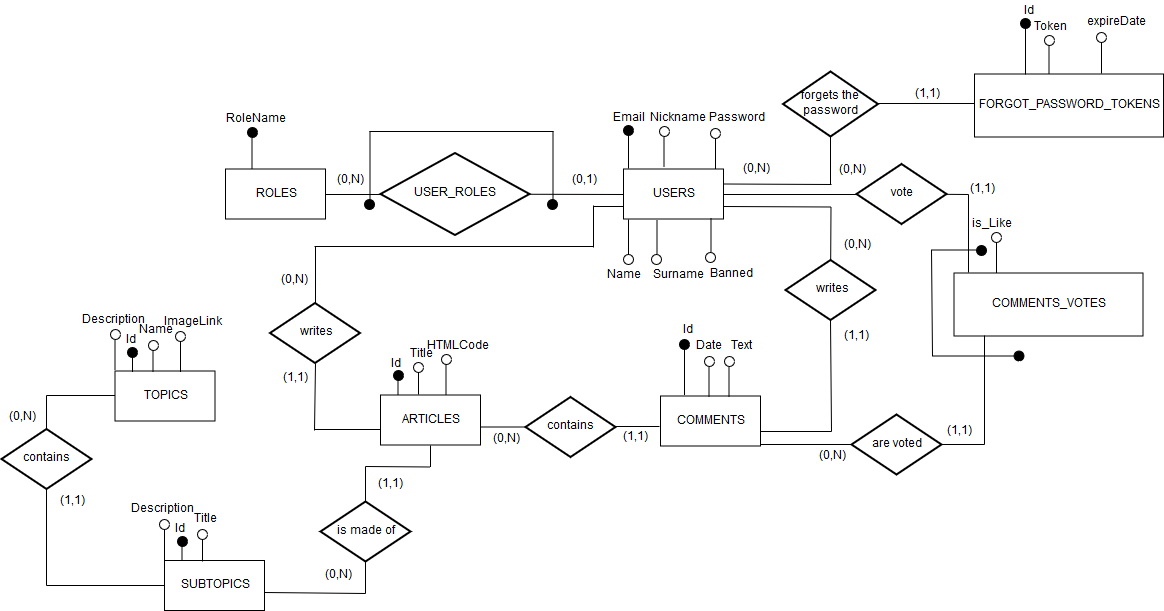
\includegraphics[scale=0.34]{img/ER_DevSpace.png}
		\caption{Diagramma ER}\label{}
	\end{figure}
	 Il database è composto da una struttura abbastanza basilare per conservare tutti i dati nella maniera più semplice possibile e per garantire facile reperibilità di ogni informazione. Le tabelle del database sono:
	\begin{itemize}
	\item tabella per gli utenti, chiamata \textbf{USERS}, che contiene i dettagli dell'utente come l'email e la password, più un campo che segna se quell'utente è stato bannato;
	\item \textbf{ROLES} è una tabella adibita a contenere i possibili ruoli che un utente può avere, nel nostro caso solo Amministratore;
	\item Dalla relazione \textbf{USERS} e \textbf{ROLES} nasce la tabella \textbf{USER\_ROLES} che associa un ruolo ad un utente;
	\item La tabella \textbf{TOPICS} contiene tutti i macroargomenti, particolare attenzione qui va al campo \textit{ImageLink}, che conterrà il percorso per la copertina del macroargomento caricata in "uploads/" durante la creazione;
	\item La tabella \textbf{SUBTOPICS} contiene tutti i sottoargomenti con il riferimento al macroargomento di cui fanno parte;
	\item La tabella \textbf{ARTICLES} contiene tutti gli articoli con il riferimento al sottoargomento di cui fanno parte, salvando anche chi è l'autore dell'articolo;
	\item La tabella \textbf{COMMENTS} contiene tutti i commenti, con contenuto data e autore e il riferimento all'articolo di cui ogni commento fa parte;
	\item Collegata alla tabella \textbf{COMMENTS} vi è \textbf{COMMENTS\_VOTES} che segna quando un utente mette mi piace/non mi piace ad un commento, chiaramente con un riferimento al commento originale, in modo da poter ricavare velocemente tutti i voti di un commento;
	\item Infine, la tabella \textbf{FORGOT\_PASSWORD\_TOKENS} è utilizzata per memorizzare i token di recupero password, generati quando un utente chiede l'email per recuperare la password dimenticata. Oltre al token è presente una data di scadenza, utilizzata per verificare che il token non sia più utilizzabile dopo 7 giorni. In questa tabella il \textit{token} era \textit{UNIQUE} per garantire che non potessero essercene di doppi, tuttavia la versione di SQL installata nel server di tecweb non permetteva questo poiché il campo era troppo lungo per essere \textit{UNIQUE}. L'assenza di doppioni è quindi controllata da PHP alla creazione di un nuovo token.
	\end{itemize}
	
	\subsection{Gestione Javascript}
	Per la gestione delle pagine in assenza di JavaScript sono state utilizzate principalmente due tecniche:
	\begin{itemize}
			\item l'utilizzo del tag \code{<noscript>} che permette di definire porzioni di codice HTML che verranno interpretate dal browser solamente in caso JavaScript fosse disattivato.
			\item l'utilizzo di una semplice ma efficace tecnica che permette di definire del codice CSS che verrà interpretato dal browser solamente in caso JavaScript sia attivato. Questa tecnica consiste nel:
			\begin{itemize}
				\item definire all'interno del file CSS principale solo ed esclusivamente il codice che dovrà essere eseguito in assenza di JavaScript;
				\item in un secondo file definire il codice CSS che al contrario verrà eseguito solo ed esclusivamente nel caso in cui JavaScript sia abilitato. \textbf{Nota}: è sufficiente ridefinire solo i blocchi css che si vogliono sovrascrivere e non l'intero codice CSS;
				\item Tramite un apposita funzione JavaScript viene effettuato l'append di quest'ultimo foglio di stile nel tag \code{<head>} della pagina web tramite il tag \code{<link>}.
			\end{itemize}
			L'append ovviamente potrà avvenire solo ed esclusivamente con JavaScript abilitato, e ciò permette di ottenere con facilità il risultato desiderato.
	\end{itemize}
	Inoltre è importante sottolineare, ove possibile, abbiamo cercato di utilizzare i \emph{listener} invece degli attributi \code{onclick = "fn()"} per separare la struttura (HTML) dal codice JavaScript.

	\subsection{Gestione votazione commenti}
	Per evitare errori nella validazione dei contenuti è stato necessario inserire un \code{alt} univoco nelle immagini relative alla votazione dei commenti, il quale possiede la seguente struttura: \code{alt = "like button for comment with id: \emph{id} written by \emph{utente}"}. Siamo consapevoli che il messaggio possa risultare apparentemente poco significativo, però non abbiamo trovato soluzioni migliori adatte alla struttura del nostro database.
	
	
	\subsection{Ricerca dei contenuti}
	La ricerca dei contenuti è effettuata tramite la barra di ricerca, presente nella home e nelle pagine con la sidebar. Una volta inserito il termine di ricerca e inviata la richiesta alla pagina search.php, quest'ultima utilizzerà la classe \textbf{SearchManager} per ottenere i risultati di ricerca da stampare. Questa classe ha tre metodi principali, uno per ogni possibile risultato: macroargomento, sottoargomento e articolo. \\
Ognuno di questi metodi funziona in maniera abbastanza semplice: legge dal database tutti i possibili elementi e li analizza uno per uno utilizzando la funzione PHP \code{similar\_text(...)} per calcolare la somiglianza tra il termine di ricerca inserito e l'elemento del database analizzato. Quando questa somiglianza è sopra una certa percentuale il risultato viene considerato valido. \\
Per rendere il calcolo della funzione di somiglianza più efficace, sia il termine di ricerca che il termine letto da database vengono portati in minuscolo, per non svantaggiare l'utente che potrebbe dimenticarsi di utilizzare le maiuscole. Infine, abbiamo considerato una percentuale di somiglianza abbastanza bassa, precisamente del 55\%, questo perché ci siamo accorti che un valore troppo alto filtrava troppo i risultati e secondo noi è più conveniente mostrare qualche risultato in più che qualcuno in meno.
	
	\subsection{Menù e sidebar senza JavaScript}
		Come già accennatto il sito si comporta bene senza JavaScript e di seguito verranno illustrati tutti i suoi usi all'interno del sito. \\
		JavaScript è stato adoperato per gestire l'apertura e la chiusura degli elenchi presenti nella sidebar e per  personalizzare la scrollbar associata ad essa al fine di migliorare l'aspetto grafico del sito. Per la scrollbar ci siamo serviti di una libreria esterna (quindi non sviluppata da noi). Tuttavia nel caso in cui non fosse disponibile, è comunque possibile utilizzare pienamente la sidebar, in quanto la scrollbar viene sostituita con quella di default e gli elenchi vengono aperti tutti automaticamente, al fine di rendere disponibile la consultazione delle voci. Per quanto riguarda i dispositivi mobili, qualora JavaScript non fosse attivato, viene utilizzata una versione del menù a tendina e della sidebar studiate appositamente. Le versioni del menù e della sidebar da utilizzare senza JavaScript vengono stampate in fondo alla pagina e sono accessibili sempre attraverso i consueti pulsanti (ovvero gli stessi utilizzati in presenza di JavaScript) che in questo caso sono delle àncore che portano alla zona della pagina in cui sono situati questi due elementi.
		Maggiori informazioni riguardanti il funzionamento nello specifico della scrollbar verranno date all'interno della sezione successiva.
	\subsection{Framework scrollbar}
	Il team ai fini di rendere la sidebar più piacevole alla vista ha scelto di adottare un framework che permette di implementare una sidebar custom. Il team dopo una approfondita ricerca, ha deciso di scegliere il framework OverlayScrollBars (disponibile al seguente indirizzo \url{https://kingsora.github.io/OverlayScrollbars}), in quanto era relativamente semplice da utilizzare e forniva una copertura pressochè totale su tutti i browser più comuni, persino sull'ormai datato Internet Explorer fino alla versione 8.
	Per applicare la scrollbar si è dovuta utilizzare la seguente istruzione definita all'interno delle API del framework:
	\[ OverlayScrollbars(element, \{ \}) \]
	dove element corrisponde all'elemento su cui si vuole applicare la scroll bar e "\{ \}" corrisponde ad una lista di possibili parametri che ai fini del progetto si è deciso di lasciare vuota.
	Si è notato inoltre che applicando la funzione precidentemente descritta direttamente sulla sidebar si presentava un conflitto tra gli stili del framework e quelli da noi descritti. Per risolvere questa problematica si è dovuto inserire un wrapper praticamente privo di stili che contenesse la sidebar ed applicare su di esso la suddetta funzione.
	Inoltre per far risaltare maggiormente i breacrumb descritti più nel dettaglio nelle sezioni precedenti si è dovuta utilizzare la seguente istruzione definita all'interno delle API del framework:
	\[ instance.scroll(element) \]
	Questa istruzione permette di scrollare automaticamente al caricamento della pagina al punto corretto nella sidebar. Più nello specifico:
	Più nello specifico instance corrisponde ad un istanza della scrollbar ritornata dall'istruzione spiegata precedentemente ed element corrisponde all' ID dell'elemento a cui si vuole scrollare.
	Inoltre si sono effettuati molti test sulle performance del sito ed è stato constatato che esse non vengono pressochè intaccate dall'utilizzo di questo framework nonostante coinvolga molto codice javascript, in quanto la scrollbar è l'ultimo componente del sito ad essere caricato e anche se non venisse caricata, il sito risulterebbe comunque navigabile.
	E' importante sottolineare nuovamente che il sito web non sia per niente dipendente da questo framework e che la sua unica funzionalità sia quella di rendere l'estetica della pagina più piacevole. Maggiori informazioni riguardo quest'ultima affermazione sono presenti nella sezione precedente.
	\section{Compatibilità}
	\subsection{Descrizione}
	In questa sezione verrà discussa la compatibilità delle tecnologie utilizzate con i browser adottati per testare il sito. Il sito è stato realizzato seguendo in parte le specifiche HTML5, concordando sull'utilizzo  di specifici tag relativi a questa versione HTML, soprattutto durante i controlli dei form.
	\subsection{Tag HTML5 utilizzati}
	\begin{itemize}
		\item Attributo \code{for} del tag \textbf{\code{<label>}}: usato per definire "label", etichette per tutti i tag che la prevedono all'interno dei form. Fornisce un miglioramento dell'usabilità per gli utenti che navigano tramite utilizzo del mouse perché attiva il controllo nel caso un utente clicchi sul testo che prevede una label;
		\item Attributo \code{type} per \code{<input>}: abbiamo utilizzato alcuni valori introdotti con HTML5 per dichiarare lo scopo di un elemento \code{<input>}. Nei form ad esempio, di login, del profile e di registrazione, è presente il \code{type="email"};
		\item Attributi \code{required} e \code{pattern} del tag \code{<input>} per sfruttare la validazione dei dati offerta da HTML5;
		\item Attributo \code{placeholder} per fornire un suggerimento su ciò che si deve inserire nei campi di input.
	\end{itemize}
	\subsection{Browser supportati}
	Il sito deve essere funzionante sul maggior numero di browser disponibili sul mercato con le versioni più recenti. I test sono stati effettuati sui seguenti browser:
		\begin{itemize}
			\item Google Chrome - Versione 72.0.3626.96 (Build ufficiale) (a 64 bit);
			\item Mozilla Firefox - Versione 65.0 (64 bit);
			\item Safari - Versione 12.0.3 (14606.4.5);
			\item Microsoft Edge - Versione 17.17134;
			\item Internet Explorer - Versione 9 e successive (11.523.17134.0).
		\end{itemize}
	Si presuppone che alcune funzionalità non si comportino allo stesso modo in tutti i browser e non siano garantite su quelli più datati. Si accerta comunque che il sito degradi in	maniera elegante sui browser più vecchi.
	\subsection{JavaScript}
	Dai test effettuati abbiamo riscontrato che il sito è utilizzabile e consultabile completamente senza l'utilizzo di JavaScript secondo le tecniche per ovviare alla sua mancanza descritte nella sezione \textbf{Sviluppo}. \\
	Alcune limitazioni:
	\begin{itemize}
		\item Non avere la possibilità di chiudere le sezioni degli argomenti nella sidebar poiché vengono aperte automanticamente per poter fruire dei contenuti;
		\item Tasto "torna su" non funzionante;
	\end{itemize}
	Siamo consapevoli di aver utilizzato molto JavaScript ma, a parte la libreria esterna per gestire la scrollbar non sviluppata da noi e utilizzata per lo stile, la maggior parte del codice riguarda ai controlli dei form client-side personalizzati (circa 600 righe sulle 800 che abbiamo scritto).
	Tutto ciò però non inficia né sull'accessibilità in quanto è stato già descritto come abbiamo gestito la sua assenza, né le prestazioni del sito in termini di caricamento e tempi di riposta come si può notare nella sezione dei test delle performance.
	
	\section{Test}
	\subsection{Accessibilità}
	Strumenti utilizzati per valutare l'accessibilità e risultati ottenuti.
	\subsubsection{Strumenti utilizzati}
		\begin{itemize}
			\item \textbf{NVDA}: screen reader gratuito reperibile al seguente indirizzo: \url{https://www.nvaccess.org/};
			\item \textbf{WebAIM Color Contrast Checker}: strumento per controllare il contrasto dei colori reperibile al seguente indirizzo: \url{https://webaim.org/resources/contrastchecker/};
			\item \textbf{Web Accessibility Checker}: strumento per valutare il grado di accessibilità di un sito secondo le linee guida WCAG 2.0 reperibile al seguente indirizzo: \url{https://achecker.ca/checker/index.php};
			\item \textbf{Total Validator}: strumento per validare le pagine e valutarne l'accessibilità reperibile al seguente indirizzo: \url{https://www.totalvalidator.com/index.html};
			\item \textbf{Colorblind Web Page Filter}: strumento per simulare il modo in cui un utente affetto da disturbi visivi quali Protanopia, Deutanopia, Tritanopia e Achromatopsia visualizza una pagina web, reperibile al seguente indirizzo: \url{https://www.toptal.com/designers/colorfilter};
			\item \textbf{Google Chrome Audits}: strumento integrato nei tools degli sviluppatori che fornisce un numero che indica il grado di accessibilità di un sito web (e anche altri parametri).
		\end{itemize}
	\subsubsection{Risultati}
		\begin{itemize}
			\item \textbf{NVDA}: nonostante la nostra prova con lo screen reader conti molto poco in termini di valutazione (infatti è stato molto difficile da utilizzare), abbiamo notato che alcune accortezze di base (come alt nelle immagini) risultano soddisfatte, e in generale il sito dovrebbe essere consultabile seppur con qualche difficoltà. Siamo comunque consapevoli di non aver potuto avere un giudizio reale sotto questo punto di vista, perciò il sito potrebbe presentare ancora molti da aspetti che devono essere migliorabili per aiutare l'accessibilità a individui che fanno uso di questo strumento;
			\item \textbf{WebAIM Color Contrast Checker}: in fase di scelta dei colori da utilizzare per foreground e background è stato utilizzato questo strumento al fine di assicurarci che il rapporto dei contrasti fosse almeno pari a 7:1. Pertanto tutti i colori utilizzati sono in linea con WCAG 2.0 AAA;
			\item \textbf{Web Accessibility Checker}: tutte le pagine sono state sottoposte ai test effettuati da questo strumento (selezionando WCAG 2.0 AAA come riferimento) e non sono stati segnalati errori di alcun tipo. Le uniche segnalazioni sono miglioramenti che possono essere apportati per migliorare ancora di più il grado di accessibilità;
			\item \textbf{Total Validator}: tutte le pagine sono state sottoposte a questo validatore, le cui risposte generate sono positive sia in termini di validazione HTML sia per quanto riguarda l'accessibilità (WCAG 2.0 AAA). Le uniche segnalazioni individuate sono alcuni \emph{warning} rimasti irrisolti, i quali però non inficiano sulla validità e correttezza delle pagine;
			\item \textbf{Colorblind Web Page Filter}: il simulatore di daltonismo che permette di simulare il modo in cui gli utenti affetti da Protanopia, Deutanopia, Tritanopia e Achromatopsia, visualizzano il sito è stato utilizzato su tutte le pagine del sito. Pur essendo questo aspetto difficile da valutare se non svolto da individui affetti dalle patologie già citate, il sito ci è sembrato comunque accessibile e usabile in quanto non abbiamo realizzato pagine molto colorate, infatti i colori più utilizzati sono il bianco, il grigio e il blu per i pulsanti. Inoltre i link (in particolare quelli per navigare all'interno del sito) sono tutti sottolineati e quindi ciò aiuta a identificarli anche laddove i colori non riescano;
			\item \textbf{Google Chrome Audits}: questo strumento, integrato nella toolbar degli sviluppatori di Google Chrome, riporta alcuni parametri principali (Performance, Accessibilità, SEO). Per quanto riguarda l'accessibilità, il sito ha riportato un punteggio pari a 100/100. Tuttavia siamo consapevoli che questo strumento non è preciso ed esaustivo come altri già citati ai punti precedenti, come Web Accessibility Checker e Total Validator.
		\end{itemize}
	
	\subsection{Usabilità}
	Strumenti utilizzati per valutare l'usabilità e risultati ottenuti.
	\subsubsection{Strumenti utilizzati}
		\begin{itemize}
			\item \textbf{Google Mobile Friendliness Test}: strumento offerto da Google per testare l'usabilità di un sito su dispositivi mobili, reperibile al seguente indirizzo: \url{https://search.google.com/test/mobile-friendly};
			\item \textbf{Test umano}: il sito è stato utilizzato da persone esterne allo sviluppo per ottenere un parare oggettivo. Inoltre è stato utile per osservare la facilità con cui navigavano e il tempo necessario per capire dove trovare le informazioni.
		\end{itemize}
	\subsubsection{Risultati}
		\begin{itemize}
			\item \textbf{Google Mobile Friendliness Test}: il sito è stato valutato positivamente, pertanto risulta essere ottimizzato per i dispositivi mobili;
			\item \textbf{Test umano}: coloro che hanno utilizzato il sito non hanno trovato difficoltà nella navigazione e si sono trovati davanti un sito a detta loro "familiare", questo indica che la struttura scelta è abbastanza affermata e quindi facile da imparare e ricordare.
		\end{itemize}
	\subsection{Performance}
	Strumenti utilizzati per valutare le performance e risultati ottenuti.
	\subsubsection{Strumenti utilizzati}
		\begin{itemize}
			\item \textbf{Google PageSpeed Insights}: strumento offerto da Google per testare le performance di un sito web, reperibile al seguente indirizzo: \url{https://developers.google.com/speed/pagespeed/insights/?hl=it};
			\item \textbf{Google Chrome Audits}: strumento integrato nei tools degli sviluppatori che fornisce informazioni sulle performance di un sito web (e anche altri parametri).
		\end{itemize}
	\subsubsection{Risultati}
		\begin{itemize}
			\item \textbf{Google PageSpeed Insights}: i test con questo strumento hanno ottenuto un punteggio ottimo, compreso tra 98 e 100;
			\item \textbf{Google Chrome Audits}: i test con questo strumento hanno ottenuto un punteggio ottimo, compreso tra 95 e 100.
		\end{itemize}
	\textbf{Nota}: i valori di questi test possono variare a seconda di diversi fattori, ad esempio la velocità della connessione.
	\subsection{Validazione}
	Strumenti utilizzati per validare i documenti e risultati ottenuti.
	\subsubsection{Strumenti utilizzati}
	\begin{itemize}
		\item \textbf{Total Validator}: strumento per validare le pagine e valutarne l'accessibilità reperibile al seguente indirizzo: \url{https://www.totalvalidator.com/index.html};
		\item \textbf{Validatore HTML}: validatore di documenti HTML offerto dal W3C, reperibile al seguente indirizzo: \url{https://validator.w3.org/};
		\item \textbf{Validatore HTML\&CSS}: validatore di documenti HTML compresi di CSS offerto dal W3C, reperibile al seguente indirizzo: \url{https://jigsaw.w3.org/css-validator/}
	\end{itemize}
	\subsubsection{Risultati}
		\begin{itemize}
			\item \textbf{Total Validator}: le pagine del sito sono state tutte validate e non presentano errori;
			\item \textbf{Validatore HTML}: le pagine del sito sono state tutte validate e non presentano errori;
			\item \textbf{Validatore HTML\&CSS:} i fogli di stile sono stati validati e non presentano errori.
		\end{itemize}
	
	\section{Suddivisione dei ruoli}
	Il team ha strutturato in modo equo il carico di lavoro per ciascun componente del team. Inoltre abbiamo fatto in modo, per quanto possibile, di sviluppare individualmente ciascun aspetto del sito (front-end e back-end). Di seguito la suddivisione principale del lavoro:
	\begin{itemize}
		\item \textbf{Giacomo Barzon}: front-end relativo alla gestione dei contenuti e della homepage con relative funzionalità JavaScript;
		\item \textbf{Francesco De Filippis}: struttura base hompage e back-end (gestione utenti e funzionalità associate);
		\item \textbf{Giacomo Greggio}: front-end relativo alla gestione dei contenuti, fogli di stampa e alcune funzionalità JavaScript;
		\item \textbf{Michele Roverato}: struttura base pagine articoli e back-end (gestione contenuti e databse).
	\end{itemize}
	Ci teniamo a precisare che, nonostante dalla suddivisione non risulti che tutti abbiano sviluppato ciascun aspetto del sito, ogni membro del team ha utilizzato in parte tutte le tecnologie.

\end{document}
